\section{Results} % (fold)
\label{sec:results}

As the chapters above have shown there are very different aspects that a company like AirBnB wants to collect and analyse from it's active users. These aspects can be summarised into the following categories of the Trinity Approach:

\begin{itemize}
    \item \textbf{Behavior}: First of all they will collect clickstream data to figure out about the behavior of visitors of their site. This massive amount of quantitative data will allow them to better understand how their users interact with the site and infer their intentions. 
    \item \textbf{Outcomes}: Based on that information AirBnB can also analyse what the visitors were finally doing on their site and if they have completed their task successfully. The most important part of the outcome analysis is the conversion rate and the profit. AirBnB needs to identify, if the user behaviour lead from the intention of booking to the certainty of booking, because it is the main source of income and thereby the purpose of the website from an economical point of view. 
    \item \textbf{Experience}: Although visitors might be able to complete the task on the site successfully the user experience on the site might not be optimal. Users could not find the available options at the specific point in the workflow or might not even know how to proceed on the site. At the end this could lead to unsatisfied customers that will loose interest in using the site. To prevent this worst-case from happening AirBnB will also qualitative data from surveys, interview and usability tests to figure out if and how to improve the experience on the site.
\end{itemize}

\begin{figure}[H]
\centering
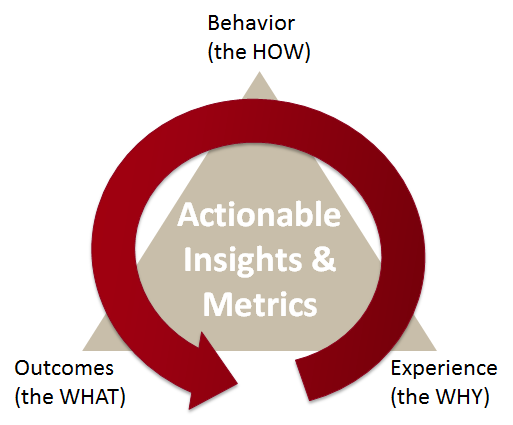
\includegraphics[width=0.6\textwidth]{assets/trinity_strategy.png}
\caption{Trinity Approach}
\label{fig:trinity}
\end{figure}

All those points are strongly related to one another and can be seen as an never-ending circle (Figure \ref{fig:trinity}). Without the clickstream data of the behavioral model (resembling the ''how" user interact) it would not be possible to check for the outcomes (showing the ''what" they have achieved at the end). These information are of huge benefit to design the questionaires and usability tests to figure out the ''why" they might succeed or fail in specific tasks. Based on those results AirBnB can further improve their web site and start this process anew to check if the changes will make any difference to the user behavior, outcome and experience. 



% section results (end)